% --------------------------
% ---- DECLARE PACKAGES ----
% --------------------------
\documentclass[a4paper, oneside, openright]{book}
\usepackage[T1]{fontenc} % Font encoding, T1 = it
\usepackage{lmodern}
\usepackage{multicol} % Per il frontespizio
\usepackage[utf8]{inputenc} % Input encoding - per caratteri particolari
\usepackage[english,italian]{babel} % Lingua principale italiano, con parti in inglese
\usepackage{blindtext} % Per la generazione di paragrafi lorem ipsum
\usepackage{graphicx} % Per includere immagini esterne
\usepackage[a4paper,top=2.5cm,bottom=2.5cm,left=3cm,right=3cm]{geometry} %impaginazione e margini documento
\usepackage[fontsize=13pt]{scrextend} %dimensione font
\usepackage{graphicx}
\usepackage[parfill]{parskip} % Disabilita l'indentazione dopo essere andati a capo
% \usepackage[hang,flushmargin]{footmisc} % Disabilita l'indentazione nelle footnotes
\usepackage{titlesec}
\usepackage{minted} % Per i blocchi di codice
\usepackage{float}
\usepackage[font=scriptsize, skip=5pt]{caption} % Spazio tra la caption e l'immagine
\usepackage[backend=biber, style=numeric, backref=true,defernumbers=true]{biblatex}
\usepackage[immediate]{silence}
\WarningFilter[temp]{latex}{Command} % silence the warning
\usepackage{sectsty}
\DeactivateWarningFilters[temp] % So nothing unrelated gets silenced
\usepackage{hyperref} % Rende l'indice cliccabile
\usepackage[justification=centering]{caption} % Per centrare le captions
\usepackage{csquotes} % Dipendenza di babel
\usepackage[bottom]{footmisc} % Posiziona le footnotes alla fine della pagina

% ------------------------
% ---- DOCUMENT SETUP ----
% ------------------------
\pagestyle{plain}
\raggedbottom % Se la pagina non è completa, lascia lo spazio alla fine

\titleformat{\chapter}[display]
    {\normalfont\huge\bfseries}{\chaptertitlename\ \thechapter}{10pt}{\LARGE}
\titlespacing*{\chapter}{0pt}{0pt}{20pt}
\chaptertitlefont{\fontsize{22pt}{30pt}\selectfont}

\hypersetup{ % Setup dell'aspetto dei link
    colorlinks,
    citecolor=black,
    filecolor=black,
    linkcolor=black,
    urlcolor=black
}

% \renewcommand{\footnoterule}{ % Rende la linea delle footnotes larga tutta la pagina
%   \kern -3pt
%   \hrule width \textwidth height 1pt
%   \kern 2pt
% } 
\renewcommand{\footnotesize}{\fontsize{11pt}{13pt}\selectfont} % Imposta la dimensione del testo delle footnotes
\setlength{\footnotesep}{0.5cm} % Imposta lo spazio fra e singole footnotes
\setlength{\skip\footins}{1.5cm} % Imposta lo spazio fra il corpo e le footnotes

\DeclareUnicodeCharacter{02BC}{}

% ------------------------
% ---- DOCUMENT START ----
% ------------------------
\addbibresource{bibliography.bib} % Importiamo la bibliografia
\begin{document} % Inizio documento
\pagenumbering{gobble} % Disabilita numerazione pagine
\begin{titlepage}
\begin{figure}[!htb]
    \centering
    
\includegraphics[width=5cm]{Immagini/uninsubria-logo.png}
\end{figure}

\begin{center}
    \Large{\textbf{UNIVERSITÀ DEGLI STUDI DELL'INSUBRIA}}
    \vspace{3mm}
    \\ \normalsize{DIPARTIMENTO DI SCIENZE TEORICHE E APPLICATE}
    \vspace{6mm}
    \\ \normalsize{CORSO  DI STUDIO TRIENNALE  IN}
    \\  \normalsize{\textbf{INFORMATICA}}
    \vspace{13mm}
    % \\ \normalsize{Tesi  di Laurea}
\end{center}

\vspace{10mm}
\begin{center}
    \LARGE{\textbf{Sviluppo di un sistema embedded per il controllo della temperatura in camera di collaudo.}}
\end{center}

\vspace*{\fill}

\begin{minipage}[t]{1\textwidth}
    \begin{multicols}{2}
    	{\normalsize{\textbf{Relatore:}}{\normalsize\vspace{1mm}
        \\ \normalsize{Prof. Carlo Dossi }}} \\ 

        % {\normalsize{\textbf{Co-relatore:}}{\normalsize\vspace{1mm}
        % \\ \normalsize{Prof. Luca Verdi }}} \\
        
         \columnbreak
         \columnbreak

         \begin{flushright}
            {\normalsize{\textbf{Tesi di Laurea di:}}{\normalsize\vspace{1mm}
            \\ \normalsize{Mattia Papaccioli}\\
            \normalsize{Matricola  747053 }}} \\
         \end{flushright}
    \end{multicols}
\end{minipage}

\begin{center}
    {\normalsize{\textbf{Anno accademico:}}{\normalsize\vspace{1mm}
    \\ \normalsize{2025/2026}}}  
\end{center}

\end{titlepage}
 % PAGINA FRONTESPIZIO
\cleardoublepage
\thispagestyle{empty}
\vspace*{\stretch{7}}
\begin{flushright}
\itshape Lorem ipsum, dolor sit \\
amet, consectetuer adipiscing elit.  \\ \vspace{5mm}
Praesent imperdiet mi nec ante \\
donec ullamcorper, felis non sodales.
\end{flushright}
\vspace*{\stretch{2}}
\cleardoublepage % PAGINA DEDICA
\tableofcontents  % Genera l'indice
\newpage % Nuova pagna
\pagenumbering{arabic} % Riabilita la numerazione in modo che cominci dal primo capitolo
\setcounter{chapter}{0} % Fa risultare l'introduzione come capitolo 0
% ------------------
% ---- CHAPTERS ----
% ------------------
\chapter{Introduzione}
Lorem Ipsum \cite{defusco}
 dolor sit amet \cite{Axa}.
Consectetuer adipiscing.\footnote{Lorem ipsum dolor sit amet, consectetuer adipiscing elit. Etiam lo-
bortis facilisis sem. Nullam nec mi et neque pharetra sollicitudin. Praesent
imperdiet mi nec ante. }

\begin{minted}{java}
// Hello.java
import javax.swing.JApplet;
import java.awt.Graphics;

public class Hello extends JApplet {
    public void paintComponent(Graphics g) {
        g.drawString("Hello, world!", 65, 95);
    }    
}
\end{minted}

\Blindtext

\begin{figure}
    \centering
    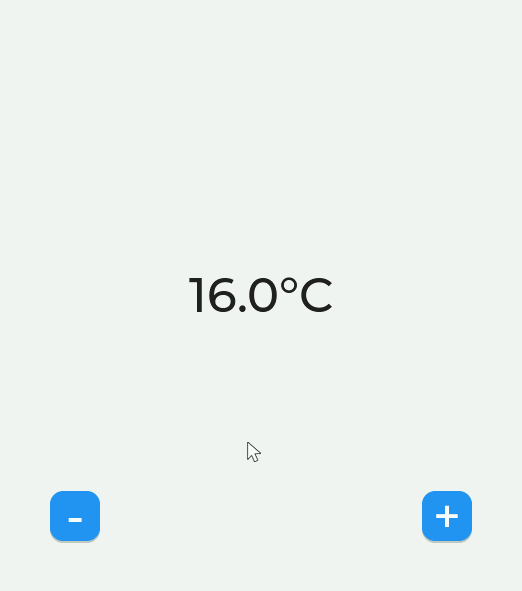
\includegraphics[width=15cm]{Immagini/lvgl-gui.png}  
    \caption{Interfaccia grafica per il controllo della temperatura}
\end{figure}

\blinddocument % Genera paragrafi e contenuti placeholder
\chapter{Conclusione}

\Blindtext



% ----------------------
% ---- BIBLIOGRAPHY ----
% ----------------------
\backmatter
\sloppy % serve a non far andare i link oltre ai margini
\printbibliography[heading=bibintoc, title=Bibliografia]
% \printbibliography[type=online, heading=bibintoc, title=Sitografia]

% ----------------------
% ---- DOCUMENT END ----
% ----------------------
\end{document} % Fine documento
